
\chapter{Sistemas HAR }

\label{chap4:sistemas-de-reconocimiento}

\section{Introducción}

\label{sec41:introduccion}El diseño de sistemas con conocimiento
del contexto promueven una interacción novedosa con los usuarios y
diversas aplicaciones en las áreas de ambientes inteligentes, repuesta
a emergencias, vigilancia y otros \cite{Choudhury2008}. Un sistema
con la capacidad de reconocer las actividades humanas por medio del
uso de sensores empotrados posee mecanismos para crear aplicaciones
de cuidado personal, salud y asistencia inteligente. El requerimiento
primordial de un sistema con una aplicación de contexto es que este
pueda ser portado continuamente como atuendo de sus usuarios (un sistema
\abbr{Wearable}). Por lo tanto, un sistema que acompaña continuamente
al usuario puede interaccionar oportunamente con el mismo ya que este
tiene la capacidad de observar en tiempo real las acciones de su portador.
La ventaja adicional de un sistema de este tipo es que puede ser desactivado
fácilmente o removido de la actividad diaria de su usuario.

En este capítulo se definen los componentes principales de un sistema
de reconocimiento de actividades humanas (sistemas \abbr{HAR}). El
objetivo principal del sistema \abbr{HAR}en conjunto es proveer módulo
base para aplicaciones novedosas de contexto. El módulo debe ser capaz
de reconocer varias actividades realizadas rutinariamente de diferentes
maneras, por diferentes usuarios y en diferentes condiciones contextuales.
Las funciones principales de los componentes descritos en la primera
sección exponen los mecanismos para implementar los mismos en base
trabajos relacionados de \abbr{HAR} \cite{Choudhury2008,ReyesOrtiz2015}. 

La última sección, enumera los requisitos no funcionales para lograr
una aplicación de contexto móvil y ubicua. Por un lado, las características
esperadas en una aplicación de esta naturaleza, y por el otro los
requisitos técnicos de los dispositivos móviles y los sensores empotrados
utilizados como instrumentos\footnote{\emph{hardware}} de implementación.

\section{Arquitectura del sistema}

\label{sec42:componentes}El diseño de la arquitectura de componentes
de un sistema \abbr{HAR} se rige de acuerdo a las guías de implementación
de una aplicación de aprendizaje automático (\abbr{ML}). De acuerdo
al proceso definido en la sección \ref{sec262:proceso-har}, se tiene
en cuenta la misma estructura de componentes y las mismas fases de
procesamiento de información. Además, se debe contemplar que el proceso
se divide en dos etapas: la etapa de entrenamiento y la de evaluación
\cite{LaraLabrador2013}. 

Ambas etapas requieren la implementación de los mismos componentes,
pero un sistema \abbr{HAR} práctico debe contemplar principalmente
la fase de evaluación, ya que el reconocimiento de actividades resulta
de una \emph{predicción} basado en un algoritmo de \abbr{ML} en-linea
(\emph{On-line learning}). Sin embargo, la etapa de entrenamiento
es un elemento clave para el sistema ya que es el punto de partida
para el \emph{aprendizaje} basado en modelo de \abbr{ML} y usualmente
se realiza bajo demanda (\emph{Off-line learning}).

Bajo el marco teórico de los sistemas \abbr{HAR} basados en \abbr{ML},
se han identificado unos componentes comunes para realizar las funcionalidades
de aprendizaje y predicción según\cite{Choudhury2008}. Un sistema
de reconocimiento de actividades posee tres componentes:
\begin{itemize}
\item un \emph{recolector }de medidas
\item un\emph{ procesador }de muestras 
\item un \emph{clasificador }de actividades
\end{itemize}
En la \figref{fig42:componentes-har} se muestra una vista general
de los componentes y sus interrelaciones. Las funcionalidades de cada
componente se describen a continuación. 

\begin{figure}[!tbph]
\centering{}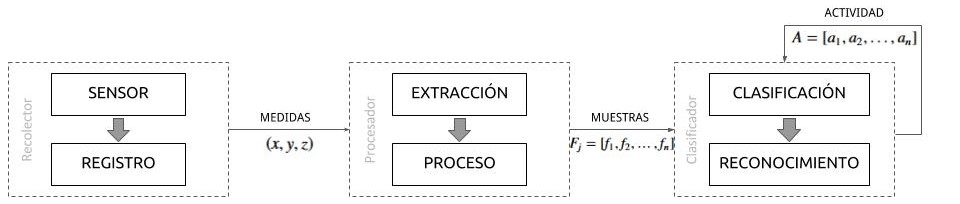
\includegraphics[width=1\linewidth]{capitulo-4/graphics/diagrama_4_1}\caption[Componentes de los sistemas HAR]{\label{fig42:componentes-har}Componentes de los sistemas \abbr{HAR}}
\end{figure}


\subsection{Recolector de medidas}

\label{sec421:recolector-datos}El recolector de datos obtiene medidas
de los sensores y continuamente registrar los datos en forma indexada
en la dimensión del tiempo. La captura de datos para los sistemas
\abbr{HAR} se realiza con instrumentos de medición apropiados: en
nuestro caso con sensores (\abbr{Wearables}, véase \ref{sec23:sensores}).
Las señales de los sensores capturan directamente de los usuarios
por medio de observaciones continuas, por lo que deben estar anexados
al cuerpo; en la cintura, la muñeca, el pectoral, los muslos o en
la cabeza \cite{Bao2004}. Adicionalmente, los sensores puede ser
portados simplemente ya están comúnmente empotrados en dispositivos
de uso regular como los teléfonos móviles modernos, relojes o lentes
inteligentes \cite{LaraLabrador2012,Choudhury2008}.

A continuación se describe el método de registro de datos en flujo
además de algunos ejemplos de variables relevantes utilizadas.

\subsubsection{Registro}

El proceso de registro consiste en capturar las señales de un sensor
y separar las medidas en una o más variables dependientes de cada
tipo de sensor. La organización de los registros se debe realizar
con respecto al tiempo. Es decir, se dispone de un flujo continuo
de datos con una marca de tiempo almacenados de manera secuencial
en un medio permanente para su posterior procesamiento. 

La marca de tiempo se mide milisegundos y dependiendo del tipo de
sensor el intervalo entre medidas de variables puede variar en el
mismo orden, Ej. con tasa de salida de \texttt{60 \abbr{Hz} }se tendrían
60 muestras en un segundo. 

Las señales capturadas de sensores se pueden clasificar en de movimiento,
entorno, fisiológicas y posición.

\subsubsection{Señales de Movimiento}

Los sensores de movimiento proveen señales altamente informativos
para las \abbr{HAR} debido a que miden las fuerzas de aceleración
y rotación en tres ejes cuando son portados por los usuarios. En esta
categoría de sensores se encuentran los acelerómetros y giroscopios. 

Los acelerómetros miden señales de acuerdo a diferentes tipos de movimientos,
incluyendo la aceleración lineal y centrípeta, la gravedad y vibración
en dos o tres dimensiones \cite{Goehl2007}. Las variables medidas
están expresadas en la magnitud de la aceleración ejercida sobre el
dispositivo con respecto la orientación del mismo (Ej. en reposo mide
$-9.8\,m\,s^{-2}$ en dirección al suelo). Representamos el atributo
medido por la aceleración con el símbolo $a$ como el vector de los
tres componentes de la aceleración en cada eje $(x,y,z)$, cada componente
esta representado por $a_{x}$, $a_{y}$ y $a_{z}$. En la Figura
\ref{fig421:muestra-ac} se muestra un ejemplo de las medidas obtenidas
por la señal del acelerómetro en una actividad determinada.

\begin{figure}[!tbph]
\begin{centering}
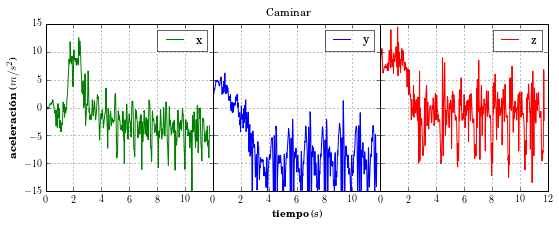
\includegraphics[width=1\columnwidth]{capitulo-4/graphics/signal_a3d}
\par\end{centering}
\caption[Señal de aceleración en tres dimensiones]{\label{fig421:muestra-ac}Señal de aceleración en tres dimensiones}
\end{figure}

Los giroscopios, o sensores de razón angular, miden señales de la
rapidez de rotación de los objetos en tres dimensiones \cite{Goehl2007}.
Las variables medidas están expresadas en velocidad angular de rotación
del dispositivo con respecto a los ejes de orientación del mismo (Ej.
en movimiento mide \foreignlanguage{english}{$-0.1\,rad\,s^{-1}$}
en relación a un eje fijo). Representamos el atributo medido por el
giroscopio con el símbolo $w$ como el vector de los tres componentes
del giro cada eje $(x,y,z)$, cada componente es representado por
$w_{x}$, $w_{y}$ y $w_{z}$. 

En el la Tabla \ref{tab421:ex-signal} se muestra un ejemplo de las
medidas registradas por la señal del acelerómetro en una ventana de
tiempo dada.

\begin{table}[!tbph]
\begin{centering}
\begin{tabular}{|c|c|c|c|}
\hline 
$t$ & $a_{x}$ & $a_{y}$ & $a_{z}$\tabularnewline
\hline 
\hline 
$0$ & \texttt{1.3} & \texttt{-2.1} & \texttt{0}\tabularnewline
\hline 
$1/s_{1}$ & \texttt{1.4} & \texttt{-2.3} & \texttt{0.1}\tabularnewline
\hline 
$2/s_{2}$ & \texttt{1.1} & \texttt{-2.6} & \texttt{0}\tabularnewline
\hline 
... & \texttt{...} & \texttt{...} & \texttt{...}\tabularnewline
\hline 
$t_{max}$ & \texttt{1.8} & \texttt{2.2} & \texttt{-0.4}\tabularnewline
\hline 
\end{tabular}
\par\end{centering}
\caption[Ejemplo de señales medidas de aceleración]{\label{tab421:ex-signal}Ejemplo de señales medidas de aceleración}
\end{table}

Las ventajas de los sensores de movimiento es su amplio uso en el
reconocimiento de actividades ambulatorias \cite{Bao2004,Kwapisz2011,ReyesOrtiz2015}.
Los acelerómetros y giroscopios poseen un bajo costo asociado, bajo
consumo de energía, además de estar incluidos actualmente en los teléfonos
móviles modernos. También, varios trabajos publicados e implementados
reportan una alta precisión en el reconocimiento de actividades \cite{Bao2004,LaraLabrador2012}.

\subsubsection{Señales de Posición}

Los sensores de posición proveen señales con información adicional
que pueden ser utilizados para las \abbr{HAR} y aplicaciones de contexto
con servicios basados en localización. En esta categoría están los
sensores de orientación (o brújula), magnetómetros y \abbr{GPS}\cite{Google2016s}.

Las señales del \abbr{GPS} permiten acceder a las coordenadas geográficas
globales así como el modo de transporte de un individuo, de acuerdo
a la velocidad estimada. Los teléfonos móviles modernos están equipados
con dispositivos \abbr{GPS} además de poder estimar con buena precisión
las coordenadas de acuerdo a la red celular \abbr{GSM}/\abbr{GPRS}
y redes \abbr{WIFI} de corto alcance. La señal de localización se
miden por medio de dos variables, latitud y longitud en la unidad
de radianes (Ej. latitud $-57.2322\,rad$ y longitud $-25.3442\,rad$).

Sin embargo, los dispositivos \abbr{GPS} tienen cobertura limitada,
ya sea por la dificultad de señal dentro de edificaciones, o sin servicio
de red celular o \abbr{WIFI}, como también el alto consumo de energía
para aplicaciones que rastrean la localización en tiempo real. La
localización particularmente es información sensible para los usuarios
ya que se debe tener especial atención a no comprometer la privacidad
de los datos y el consentimiento del usuario que permita ser rastreado
\cite{LaraLabrador2013}.

\subsubsection{Señales del Ambiente}

Los sensores de ambiente miden varios atributos del entorno que rodea
al usuario. Algunas señales como la temperatura del aire, presión
atmosférica, iluminación, humedad, y el ruido pueden proveer información
de utilidad para conocer mejor el habitad particular de un usuario.
En esta categoría están los barómetros, fotómetros, termómetros y
micrófonos.

Los sensores de ambiente solos no proveen información suficiente ya
que los individuos pueden realizar las actividades bajo diversas circunstancias
contextuales en términos de clima, ruido o iluminación. Por lo tanto
estos sensores pueden utilizarse de manera complementaria para detectar
sugestiones adicionales, Ej. el usuario está en el exterior de acuerdo
a la luminosidad, o se encuentra descansando debido a un nivel de
sonido y luminosidad baja \cite{LaraLabrador2013}.

\subsubsection{Señales de Fisiológicas}

Los sensores fisiológicos proveen señales de signos vitales de un
individuo. La información sobre el ritmo cardíaco, tasa de respiración
y temperatura del cuerpo podrían ser combinados para enriquecer el
contexto durante el reconocimiento en ciertas aplicaciones específicas
como las orientadas a la salud.

\subsection{Procesador de muestras}

\label{sec422:proceso-se=0000F1ales}Proceso de señales en bruto para
adecuarlos muestras con variables significativas que permitan discriminar
las actividades a reconocer

\subsubsection{Etiquetado}

\subsubsection{Filtro de Señal}

\subsubsection{Muestreo}

\subsection{Clasificador de actividades}

\label{sec423:clasificador}Utiliza las muestras extraídas para construir
un modelo e predecir qué actividad probable está realizando un individuo
en un determinado instante.

\subsubsection{Clasificación}

\subsubsection{Reconocimiento}

\section{Capacidades deseables}

\subsection{Características no funcionales}

\label{sec431:caracteristicas}Existen un conjunto de características
deseables que deben ser satisfechas para la construcción efectiva
de los sistemas de reconocimiento. Estas características abordan cuestiones
de diseño importantes que conciernen a la calidad y al funcionamiento
del sistema:
\begin{enumerate}
\item Portabilidad, el sistema utiliza sensores adjuntos a los individuos
(Ej. el acelerómetro) y no deben obstruir las actividades cotidianas
de los usuarios durante su uso. El fin es de evitar que se afecte
la adopción masiva del sistema. 
\item Conectividad, el sistema debe transmitir de manera confiable los datos
recolectados y/o procesados a algún componente desplegado de forma
remota. 
\item Almacenamiento, el sistema debe persistir los datos recolectados y/o
procesados de manera local en el dispositivo móvil con el fin de mantener
la calidad y minimizar la cantidad transferida a otros componentes.
\item Procesamiento, el sistema debe procesar y transformar los datos en
bruto para producir información relevante para el reconocimiento de
actividades.
\item Ubiquidad, el sistema debe operar en cualquier condición y contexto
en que la persona se encuentre sin interferir u obligar al usuario
a interactuar con el sistema.
\item Uso de energía, el sistema debe preservar el uso de energía en los
dispositivos móviles que están implementados. La lectura de datos,
el procesamiento y la conectividad no deben incurrir en gastos excesivos
de energía para que el sistema pueda operar.
\item Privacidad, el sistema debe mantener de manera confidencial los datos
recolectados y/o producidos durante la adopción masiva del sistema,
además de alertar sobre la utilización de datos sensibles que requieran
el consentimiento del usuario.
\end{enumerate}

\subsection{Dispositivos móviles}

\label{sec432:dispositivos-moviles}Descripción técnica de dispositivos
móviles: procesador, memoria, sensores y almacenamiento

\subsubsection{Teléfonos móviles}

\subsubsection{Relojes inteligentes}

\subsection{Sensores empotrados}

\label{sec433:sensores-empotrados}Descripción técnica de los sensores
de aceleración, variables, orientación en dispositivo, unidades de
medida, precisión vs consumo.

\subsubsection{Acelerómetro}

\subsubsection{Giroscopio}

\subsubsection{GPS/WIFI}

\section{Conclusión}

Resumen
